\section{\droidxpflow}

In this section we detail some design decisions
related to \droidxpflow, which uses \droidxp~\cite{DBLP:conf/scam/CostaMCMVBC20} to
collect network traffic of Android apps while
using a test case generation tool and leverages
machine learning algorithms to classify the
apps as malware or non-malware. Since \droidxpflow
relies on ML algorithms, we organize this section
according to typical ML stages: data collection,
pre-processing, and 
feature extraction (see Figure~\ref{fig:arq}).


\begin{figure*}[h]
  \centering
  
    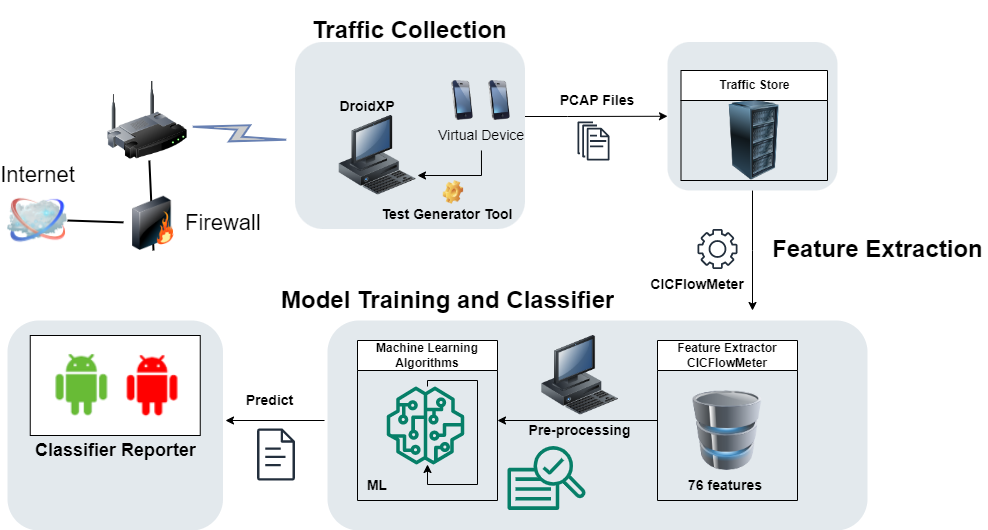
\includegraphics[width=0.80\textwidth]{image/archic.png} \\[\abovecaptionskip]
    
  \caption{Architecture of the \droidxpflow designed for malware detection}\label{fig:arq}
\end{figure*}

\subsection{Data Collection}

The DroidXP~\cite{DBLP:conf/scam/CostaMCMVBC20} tool was initially designed to compare test case generation tools in terms of identifying malicious app behaviors using the \mas. This makes it a relevant tool forautomating data collection using dynamic analysis.% , following the steps outlined below:
For our study, we extended the original version of \droidxp by adding new features to its execution phase. This extension (\droidxpflow) now uses the TcpDump tool
to collect both inbound and outbound network traffic. The \droidxpflow extension allow us to capture data for network traffic in the PCAP format~\cite{DBLP:conf/iv/UhlarHR21}.
A PCAP file contains copies of network packets, enabling dynamic analysis of both payloads and packet headers~\cite{DBLP:conf/iv/UhlarHR21}. Since storing
and processing PCAP files is a resource-intensive process, \droidxpflow only performs an analysis of network flow segments, rather than analyzing all data available in the PCAP
files. As such, we pre-process the PCAP files to extract the most relevant features for our study, using the CICflowMeter tool~\cite{DBLP:conf/icissp/LashkariDMG17} software,
as we detail next.


% \begin{enumerate}[1.]
%  \item \textbf{Instrumentation}:  All apps analyzed are instrumented to collect relevant information before execution. In the background, DroidXP leverages DroidFax~\cite{DBLP:conf/icsm/CaiR17a} to gather static information about the apps being analyzed.
 
%    %\todo[inline]{Confuso essa parte inicial do texto ``As statistical result show that \ldots''. Na verdade, o par\'{a}grafo inteiro est\'{a} super confuso. Eu diria que toda essa se\c c\~{a}o MAS Data Collection deveria ser re-escrita. Quem \'{e} 'the author'?}
   
%  \item \textbf{Execution}: DroidXP installs the instrumented versions of the apps on an Android emulator and restarts it before the actual execution. It then initiates a test case generation tool to execute all the apps and collect the dynamic data from the pre-programmed executions setup.
  
% %\todo[inline]{A se\c c\~{a}o \'{e} sobre data collection. Vamos simplificar essa se\c c\~{a}o, deixa-la mais atrativa para um leitor.}   

% \item \textbf{Data Collection}: At the end of the execution step, DroidXP again utilizes DroidFax, this time to compile all relevant information from the execution step, such as calls to sensitive APIs, and more. This step, and previous are crucial for dynamic analysis.
% \end{enumerate}


\subsection{Pre-processing}

\rb{Temos que explicar o porqu\^{e} da remocao dessas features. Por que elas nao sao relevantes? Acho estranho descartarmos Source IP, por exemplo}

\droidxpflow processes each resulting PCAP file, collected during the data collection stage, using the CICFlowMeter tool.
CICFlowMeter extracts feature sets in CSV format from the corresponding PCAP files, combining them into a single file that
contains a total of 86 features, including flow duration, destination port, number of transmitted bytes, and so on.
\droidxpflow discards from the analysis features that we consider irrelevant to our study, such as
Flow ID, Source IP, Destination IP, Source Port, Source MAC, Destination MAC, Protocol, and Timestamp
(resulting in 78 features).

\rb{Esse par\'{a}grafo eu trabalhei principalmente com a qualidade do texto. Tecnicamente, ainda o considero
  questionavel. Essa parte de
  Comando e Controle \ldots, por exemplo, eu optei por deixar em vermelho. Talvez o Prof. Joao Gondim possa
  melhora-lo, Handrick. Eu acho uma decis\~{a}o equivocada mantermos 4, 5 e 6. A maior parte dessa
  tr\'{a}fego \'{e} HTTPS. Qual a garantia que o protocolo 5228 tem relacao com mensageria da google}


During preprocessing, \droidxpflow discards observations where the ``Destination Port'' does not correspond to the most frequent services,
such as HTTP (and its variants) or DNS. The destination port numbers help categorize the services utilized in network traffic.
Previous studies have demonstrated the relevance of destination ports in classifying malicious behavior~\cite{DBLP:journals/compsec/UmerSB17,DBLP:journals/comsur/SperottoSSMPS10},
as they are often exploited for {\color{red}purposes such as communication with Command \& Control (C\&C) servers, carrying out exploits,
or blending in with normal traffic~\cite{DBLP:journals/comsur/SperottoSSMPS10}}. Commonly targeted ports include 80 (HTTP), 443 (HTTPS), and 53 (DNS).

Furthermore, other datasets frequently used in related research, such as CIDDS-001~\cite{Ring2017FlowbasedBD}, CICIDS17~\cite{DBLP:conf/icict/MahfouzVS19},
and CTU-13~\cite{DBLP:journals/compsec/GarciaGSZ14}, have leveraged the destination port feature for network flow classification.
Considering the significance of the Destination Port feature highlighted in these studies, along with a preliminary analysis of our datasets
(see the Section~\ref{sec:empirical-study}), we opted to filter out network traffic data that do not correspond to the six most
relevant destination ports identified in our analysis. These six ports account for $74.25\%$ of the total network traffic captured in our experiment
(see Table~\ref{tab:port}).

\begin{table}[h]
\centering
\caption{The six most relevant destination ports in our study.}
\begin{small}
\begin{tabular}{rlrl} 
\hline
Port & Description & Occurrences \\ 
\hline
443 & Hypertext Transfer Protocol Secure & 1,275,293 \\ 
53 & Domain Name System & 641,965 \\ 
80 & Hypertext Transfer Protocol & 38,830 \\ 
853 & DNS over TLS & 32,784 \\ 
5228 & Google Cloud Messaging & 26,509 \\ 
123 & Network Time Protocol & 9,179 \\ 
\hline
\end{tabular}
\end{small}
\label{tab:port}
\end{table}

\subsection{Feature Extraction}


Selecting relevant features (i.e., feature extraction) is crucial for achieving strong predictive performance in
machine learning (ML) models~\cite{DBLP:conf/ichmi/Xie22,DBLP:journals/mta/AmiriebrahimabadiM24}. Feature extraction not only
improves model accuracy but also reduces training time. However, selecting appropriate features is a challenging task that often requires domain expertise. 

To address this challenge, it can be more effective to allow the machine to learn which features are most important~\cite{DBLP:journals/spe/FallahB22}.
In this regard, \droidxpflow computes seven additional statistical features (count, minimum, maximum, average, median, variance, and skewness)
for each of the 76 original numeric features generated by CICFlowMeter from the PCAP files. These additional statistical features are then fed into the model. 
At the end of this stage, our ML models consider a total of 3,194 features (76 numeric features from CICFlowMeter $\times$ 6 protocols (destination ports) $\times$ 7 statistics),  
plus the hash ID of the Android apps and the label (i.e., malware or non-malware).

\rb{O que foi feito para diminuir o tempo de treinamento? N\~{a}o entendi bem o pr\'{o}ximo par\'{a}grafo, e est\'{a} incompleto.}

Still, high-dimensional datasets have a costly training time. To select the most relevant features and reduce their quantity, \droidxpflow \ldots
